\chapter{Theoretical Foundation}
\label{sec:theory}

A monolith is an application that has grown too big. In contrast, a microservice is just a part of a broader application that runs independently and communicates with the other parts to make a whole. Microservices are of interest today because they enable applications to scale and deploy quickly. The idea of scaling goes along with cloud computing, the idea that an application lives on remote servers and is accessed by simple clients. All this comes with the challenge of more sophisticated infrastructure and the need to manage distributed data. Therefore it is not recommended to start with a service-oriented architecture, but to destructure software on the go as scaling becomes necessary.

\begin{figure}[ht]
  \centering
  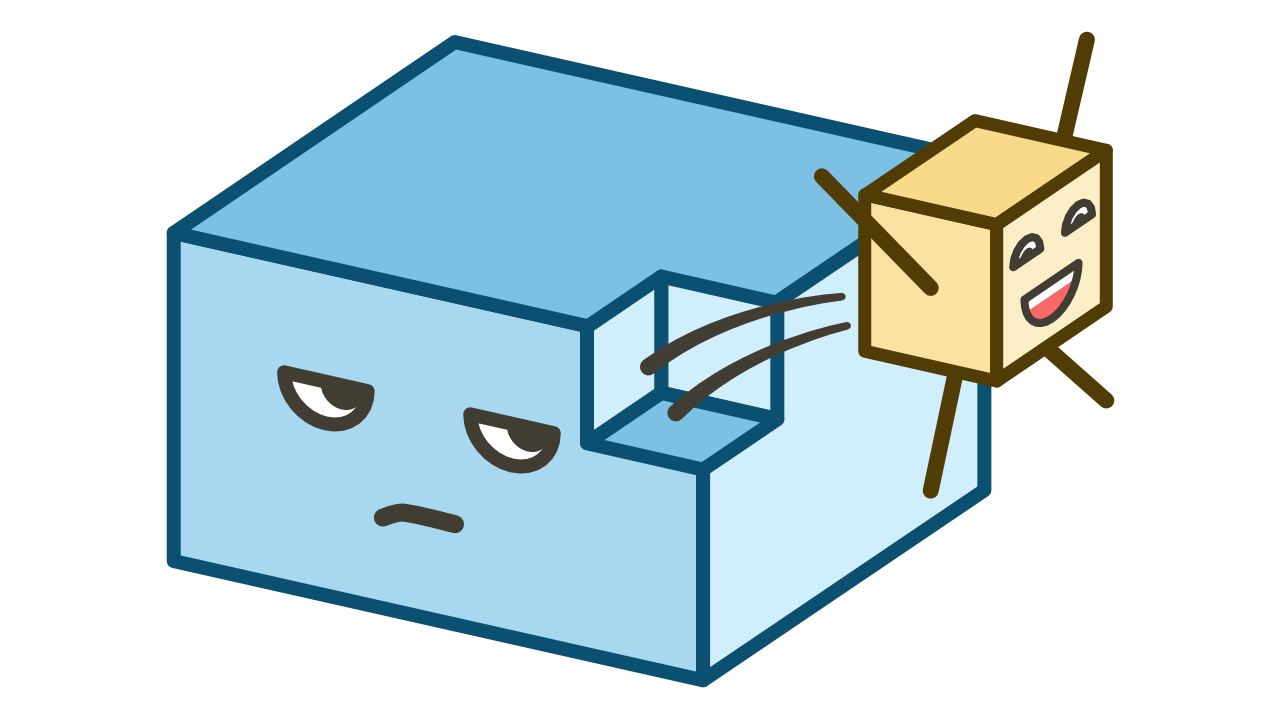
\includegraphics[width=0.4\linewidth]{assets/illustration-monolith-microservice.png}
  \label{fig:illustration-monolith-microservice}
\end{figure}


%%
%% What is a monolith?
%%
\section{What is a monolith?}

Before defining a microservice, it is advisable to understand what a monolith is since we are going to use them as a comparison. A monolith is an "application built as a single unit" ~\cite{microservices.2014}. Enterprise applications are built with a single code base that is maintained in one place by a team or several teams, all working on that one application. Three horizontal layers often separate these applications, the data persistence layer, or database, the server, and the client. The cuts for these layers run along technological boundaries instead of boundaries related to business domains. A business domain is, for example, a part of a software that takes care of user management, another domain may be concerned with all payment-related parts of the application. A layer, however, groups all part of an application that uses the same technology, for example, Java as the server-side language.

The term "monolith" describing an extensive system derives from the Unix community, which uses the term to describe systems that became too big ~\cite{raymond.2003}. When the term is used in literature or conversation, it usually describes a system that has grown very large over time and is very unwieldy for developers to work with. The development of monolith systems tends to be slow, and maintenance is high. Such systems are widespread in the industry and usually so big that several developer teams are needed to keep them running. Because a monolith is a single unit, it is very natural for its programming code to become tightly coupled between its various modules. This has the effect that programmers need more time to understand relationships inside the code than actually writing new code. Developers do not favor large applications of this type.



%%
%% What is a microservice?
%%
\section{What is a microservice?}
\label{sec:theory:what}

\begin{itemize}
  \item \done{General definition and how it works}
  \item \done{Get some ideas from the it-innovations article ...}
\end{itemize}

A microservice has four characteristics that set it apart from monoliths. They are independently deployable while monoliths can only be deplyed as one blcok. Microservices are organized around business capabilities avoiding the problem of "logic everywhere" ~\cite{microservices.2014}. Each service is governed independently simplyfing development but increasing operations overhead. And their data management is decentralized, whch poses a challenge compared to monoliths.

\subsection{Independently Deployable Services}

Every software is made up of smaller parts, usually called components. The basic concept of Object-Oriented programming, for example, is that all functions and data related to one object, like a product of a store, live in one class. The class houses the data and exposes methods for other parts of the application to interface with its data. The whole application is tied together by function calls that happen inside the memory of a physical machine.

A microservice, on the other hand, is an application that lives on a physically different machine from other services and communicates through mechanisms like an HTTP request. Services don't always have to be on separate machines, but they are always treated like closed systems, and communication happens as if they were on physically separate machines.

Changes in one part of an application that consists of components only take effect when redeploying the whole application. For monoliths, this means that even small changes relative to the entire codebase require a redeploy of the whole system. A system made up of microservices only needs to redeploy the specific service where the change was made. A change in one service may also depend on a change of another service, which means there needs to be some coordination when updating them. However, in general, a microservice is independent of its neighbors and can be deployed and, more importantly, scaled as such.


\subsection{Organized around Business Capabilities}
\label{sec:theory:what:capabilities}

In his excellent article about microservices ~\cite{microservices.2014} Martin Fowler mentions Conway's Law ~\cite{conway.1968} in regards to large applications. The law states that "any organization that designs a system [...] will inevitably produce a design whose structure is a copy of the organization's communication structure." An organization's structure for software projects often groups different technologies into layers, which leads to different teams skilled for different tasks. An example may be the backend team and the frontend team. Working cross team is usually accompanied by some red tape like budget approvals leading to teams optimizing to solve problems internally. This leads to business logic ending up in places of the system where it shouldn't.

\begin{figure}[ht]
  \centering
  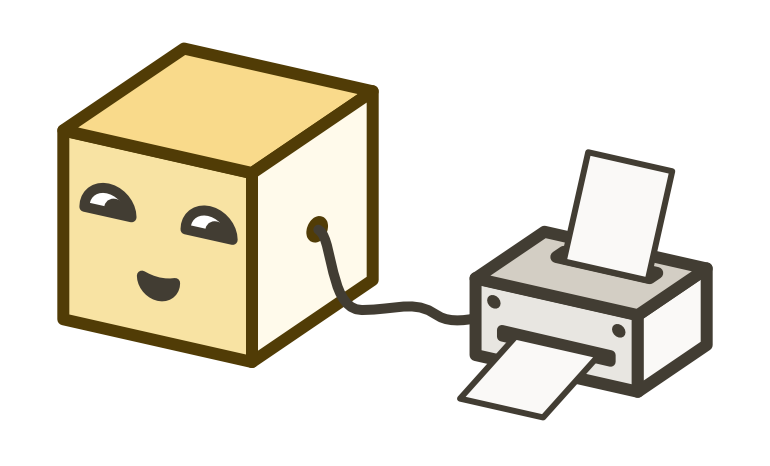
\includegraphics[width=0.4\linewidth]{assets/illustration-microservice-printer.png}
  \caption{The domain of this microservice: converting a dataset into a printed page}
\end{figure}

There are many ideas to minimize this effect, a more popular one being Domain-Driven Design ~\cite{evans.2003}. All these approaches, however, call for discipline during development. A microserver, on the other hand, is not organized around technology but a business need. For example, the hands-on part of this paper deals with a service for generating a PDF document. A team working on a microservice, therefore, needs to be cross-functional and therefore avoids organizational barriers.


\subsection{Decentralized Governance}

When splitting an application into multiple services, the developer has the choice of which technology to use. Does he want to build a simple backend API and is comfortable in JavaScript, then he could use Node.js? Is he more familiar with Java, then he could set up a simple Java Spring Framework. Or maybe he needs to use some machine learning model for image processing, in which case Python may be the best choice. Programmers prefer using the right tool for the right job. Monoliths have the inherent limitation that every part of it has to use the same technology. Of course, just because it is possible doesn't mean every service has to use different technology. Often a company is limited by the skillset present among its employees and want's to use this knowledge. Even then, every team has the freedom to define their principles and pick standards best suited for their use-case.

\begin{figure}[ht]
  \centering
  
\includegraphics[width=0.4\linewidth]{assets/illustration-monolith-hammer.png}
  \caption{Not every problem is a nail}
\end{figure}

Amazon's "You build it, you run it" methodology is an excellent example of the advantages of decentralized governance ~\cite{amazon.2015}. The idea is that the same team which builds a service is also responsible for running it. According to Stephen Orban, General Manager of an AWS Service, this "forces development teams to think about how their software is going to run in production as they design it." Leading to better software quality and more ownership among the team. Because the developers are ultimately responsible,  they make an effort to avoid bad practices. According to Orban, this even leads to more automation, because developers are inherently lazy and try to avoid repetitive tasks, and more customer satisfaction because the dev team has direct contact with the customer.


\subsection{Decentralized Data Management}
\label{sec:theory:decentralized-data}

Decentralized data management is likely the single biggest challenge with service-oriented architectures. Monoliths use a single database for the entire application, which makes data management easy. Microservices can also share a single database that would avoid the problem of having to save data in a distributed way or sync data across multiple databases, see figure \ref{fig:decentralised-data}. So why should microservices manage distributed data? The answer is encapsulation, which is a term in computer science, essentially saying that one component should handle all of its concerns internally, and another component should not know about them ~\cite{krivtsov.2019}.

\begin{figure}[ht!]
  \centering
  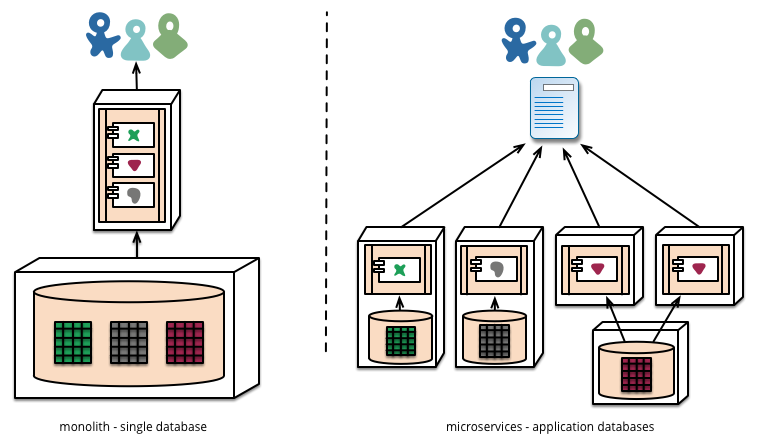
\includegraphics[width=0.7\linewidth]{assets/decentralised-data.png}
  \caption{Data management of monoliths and microservices}
  \source{https://www.martinfowler.com/articles/microservices.html}
  \label{fig:decentralised-data}
\end{figure}

Say there are two microservices, a user service and an order service. Each order is associated with one user who made the order. If both services have their database, then the order service saves the user ID in its database. If a request asks for an order bundled with the user information, then the order service has to make a request of its own to the user service to get the user information in the first place before it can bundle it with its order and send out the answer. If the user service is not available, the order service can not finish the request. Now both services access the same database, and the order service no longer needs the user service because it can merely get into the database and get the user information itself. However, this would mean that the order service knows about the internal affairs of the user service. It knows, for example, how the user table looks like. Now the two services are coupled. If a change is made to the user service, the order service also has to be adjusted. This would effectively undo the benefit of using microservices in the first place and introduce all the challenges of large monoliths into the service-oriented architecture.

Decentralized data management is the main reason why microservice architectures are not the golden bullet solution. Although the benefits of microservices outweigh monolith architectures in the long run, there is a consensus among developers that it is better to start with a monolith. Then refactor to microservices later "if you really need them in the future." ~\cite{krivtsov.2019}


%%
%% Why are microservices currently interesting?
%%
\section{Why are microservices currently interesting?}
\label{sec:theory:interesting}

\begin{itemize}
  \item \done{Application development until now with monoliths \& waterfall}
  \item \done{Avarage life and maintenance effort of a big application}
  \item \done{Rise of Agile, the Cloud and quick deployment cycles}
  \item \done{Rise of Software as a Service (SaaS), hiding complexity behind an API ~\cite[p.~359]{melzer.2010}}
\end{itemize}

Up until recently, building software worked like building a house. A team made a plan for the finished application, then developed it and then it was finished. The industry calls this the waterfall method, finishing all the plans before starting development. The finished software was one piece, and it was also sold as such. However, software is very different from real-world construction in that our digital systems became more and more complex. This complexity meant that it was necessary to keep software up to date. It meant that companies still needed to extend a finished software product by additional functions and actively maintain it. Surprisingly little thought went into the length of the life of an application, probably because the field of software development was comparatively new, and nobody knew where the journey would lead.

An excellent example of this was the fear around the Y2K bug. The only reason for the bug was that developers hadn't considered that people would use their product for so long. Today we can look back in hindsight, knowing that it is not uncommon for software to live over ten or even 20 years. Especially industry applications see long years of life.

Around the year 2001, developers started adopting agile development methods over the traditional waterfall approach ~\cite{agile.2020}. Clients demanded faster release cycles. A traditional software project can take years to completion. Stakeholders wanted prototypes, and developers needed more flexibility than before. All these factors helped agile methodologies to rise to the top until they became the de-facto way of doing software development.

Meanwhile, the internet became robust and fast enough to support decentralized computation, the cloud where more and more applications found their home. The cloud transformed the desktop computer into a client, which mainly uses services running in some datacenter instead of executing a program on its hardware. Now developers were no longer restricted by the need to distribute updates to thousands of individual machines. Upgrading an application in the cloud once was enough; every customer immediately reaped the benefits. In turn, management understood that software no longer needs to be completed before selling it to the market because it can be updated often, the more often, the better. This required developer teams to ways to shorten their development cycles more and more. Today it is normal for an application to have a pipeline for continuous deployment or continuous integration, meaning the developer can trigger a process that goes through the necessary steps to update the software automatically. This represents a considerable speedup from doing everything manually.

\begin{figure}[ht]
  \centering
  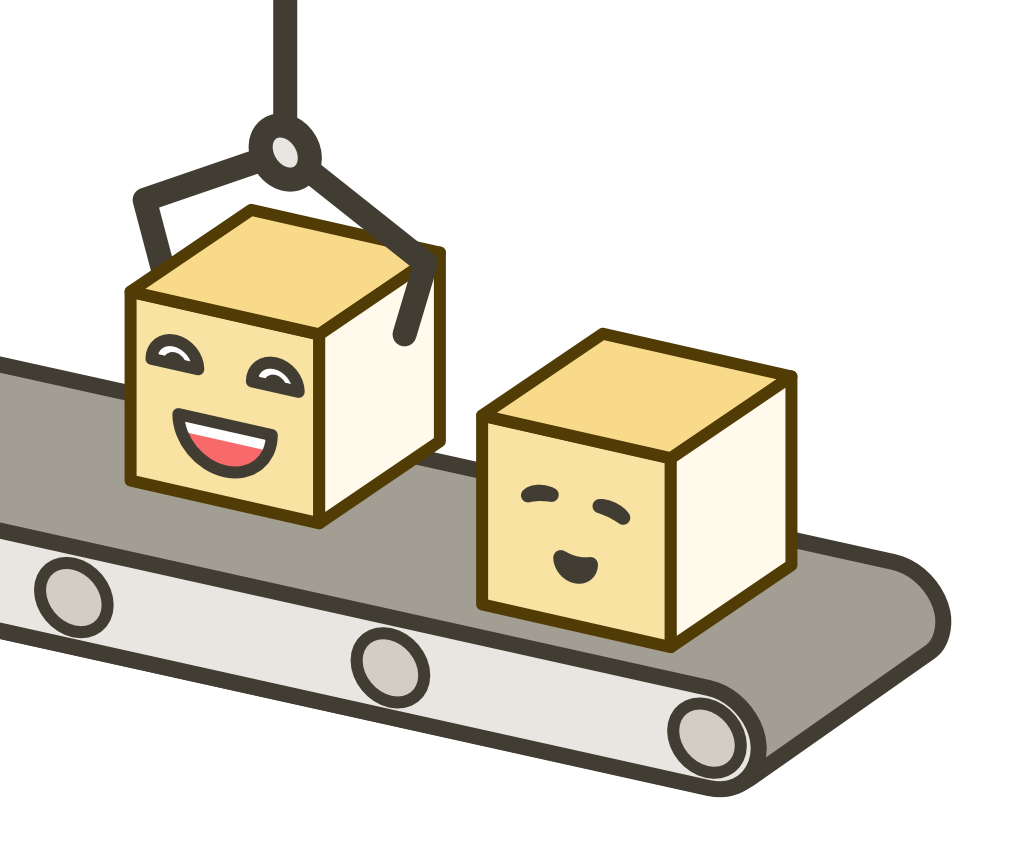
\includegraphics[width=0.4\linewidth]{assets/illustration-microservice-cd.png}
  \caption{Continuous Deployment, short CD}
\end{figure}

Before we come to the topic of microservices, we want to look at one more innovation of the computer age that is digging the grave of monolith systems. In recent years so-called Software as a Service, short SaaS, has gained considerable prevalence. The idea behind Saas is that a complex task is hidden away behind an interface. The user can pay for the service on a per-use basis, or via subscription, trigger the task and wait for the result. It makes sense because, in almost every scenario, it is cheaper to buy a software solution than to build it yourself. In today's startup world, especially, these "buy or build" decisions are essential for building complex applications with limited means. A great example of a SaaS product is the email marketing service Mailchimp that takes care of managing email subscriber lists and sending of marketing emails. Like basically every other aspect of the internet email started as a simple protocol and has developed into an incredibly complex system that makes sure that legitimate email arrives at its destination and fraudulent messages are filtered out. According to its own marketing page Mailchimp "averages \$52 ROI for every dollar spent" on email ~\cite{mailchimp.2020}. Meaning a customer can buy functionality that seamlessly integrates with his system through an interface without having to stem the cost and expertise of this functionality. Meanwhile, Mailchimp is running on a completely separate infrastructure saving the customer not only the development but also data centers, cybersecurity concerns, maintenance, and all the other new challenges the cloud brought to our modern age.

\begin{figure}[ht]
  \centering
  
\includegraphics[width=0.8\linewidth]{assets/mailchimp-brand.png}
  \source{https://mailchimp.com/about/brand-assets/}
\end{figure}

Once we reach this point, it is easy to connect the dots from third-party SaaS products to an individual application itself running as a cluster of services. In the end, the appeal for companies to break up monolith systems into service-oriented architectures lies in the idea of hiding the complexity of software behind an API\footnote{Application Processing Interface – a way to tell a service to do a specific task or request particular set of data} and looking at it as a business process ~\cite[p.~359]{melzer.2010}. A microservice essentially becomes a black box. The development team takes care that the service works and is at liberty to decide how to solve problems. To everyone else, the service represents an API that they can use to solve their issues.



%%
%% Which problem does a microservice solve?
%%
\section{Which problem does a microservice solve?}
\label{sec:theory:what-problem}

\begin{itemize}
  \item \done{Why is a microservice better than a monolith?}
  \item \done{Advantages \& Disadvantages of microservices}
  \item \done{Work/Effort of microservice compared to monolith}
\end{itemize}

Microservice architecture is the answer to the question of scalability and quick deploy cycles, which are becoming ever more critical in today's world of cloud computing. While solving these two primary concerns, it also helps with clear separation of concerns and free choice of technology and speeds up development. However, these gains come at the cost of more sophisticated infrastructure and more significant operations overhead.

\subsection{Deploy individually}

In a monolith system, change cycles are tied together. Meaning if one part of the application changes, the whole system needs to be redeployed. Redeployment not only means assigning a new version number and uploading the updated files, but it also requires the whole deploy pipeline to run. It means the entire application has to undergo testing to make sure all functions, even those not touched by the change, work as expected. Naturally, the bigger an application, the more effort the testing phase represents. If multiple teams are working on a software project, new features are usually bundled into one release and tested together. Release cycles of three months or even a year are not uncommon.

Microservices are simplifying the deployment process considerably because they physically separate individual parts of the application from one another. Meaning one service can deploy changes in isolation. Testing becomes an almost trivial task since the scope is naturally limited, and side effects are virtually non-existent. Additionally, a new feature can deploy directly to production as new features don't have to be bundled any more for the sake of testing. It means with microservices deployment is cheap and can often occur, bringing release cycles down to weeks or even days.

However, there are also new complications. If the API of a service changes, it does directly influence other services. The solution here is to version the API and support both old and new in parallel until all other services have migrated. In turn, if a new feature depends upon a new API of another service, the release has to be postponed until the API is available or deployed behind a feature switch\footnote{A feature switch is a true/false value. They can turn a feature off or on at any given time without the need to redeploy the entire application}.


\subsection{Boundaries are clear}

Tight coupling ~\cite{kaye.2003} is one of the most challenging problems of large systems. Tight coupling happens if two independent components know of and use each other's internal workings. Changing one necessitates understanding and changing the other component too. Because it is a well-known problem among programmers, there are many concepts to avoid it, like the open-closed principle. But ultimately, it needs a lot of developer discipline to keep a system loosely coupled. Especially if a system is older and has undergone many changes, tight coupling is unavoidable despite best intentions as every developer who worked on a real-world example knows very well. In monolith systems, it ultimately boils down to keeping tight coupling manageable while not wasting too much time with refactoring.

\begin{figure}[ht]
  \centering
  
\includegraphics[width=0.55\linewidth]{assets/illustration-setting.png}
  \caption{With micoservices it is easy to keep changes localized}
\end{figure}

Microservices, by design, avoid the problem of tight coupling altogether. Because individual services can only communicate through their public APIs and do not share data, see page \pageref{sec:theory:decentralized-data}, their boundaries are necessarily hard. Making changes or developing new features inside a microservice is, therefore, much faster since the developer doesn't need to worry about any side-effects. As a software developer, I know that tight coupling is one of the most significant time sinks when developing new features because it forces me to understand many parts of the application that have nothing to do with my immediate task.


\subsection{Scale the part that needs more resources}

Scaling an application is becoming a bigger requirement in today's world, where everything is in the cloud. Take Netflix, for example; it needs to serve huge amounts of data to its customers depending on both location and time. It needs to make sure that enough network bandwidth is available for the evening and weekend peaks while avoiding idle resources during the workday. Netflix also makes different shows and languages available in different geographic regions depending on the licensing rights. As sown in figure \ref{fix:netflix-architecture}, Netflix uses a whole host of services with various specifications and responsibilities ~\cite{netflix.2013}.

\begin{figure}[ht]
  \centering
  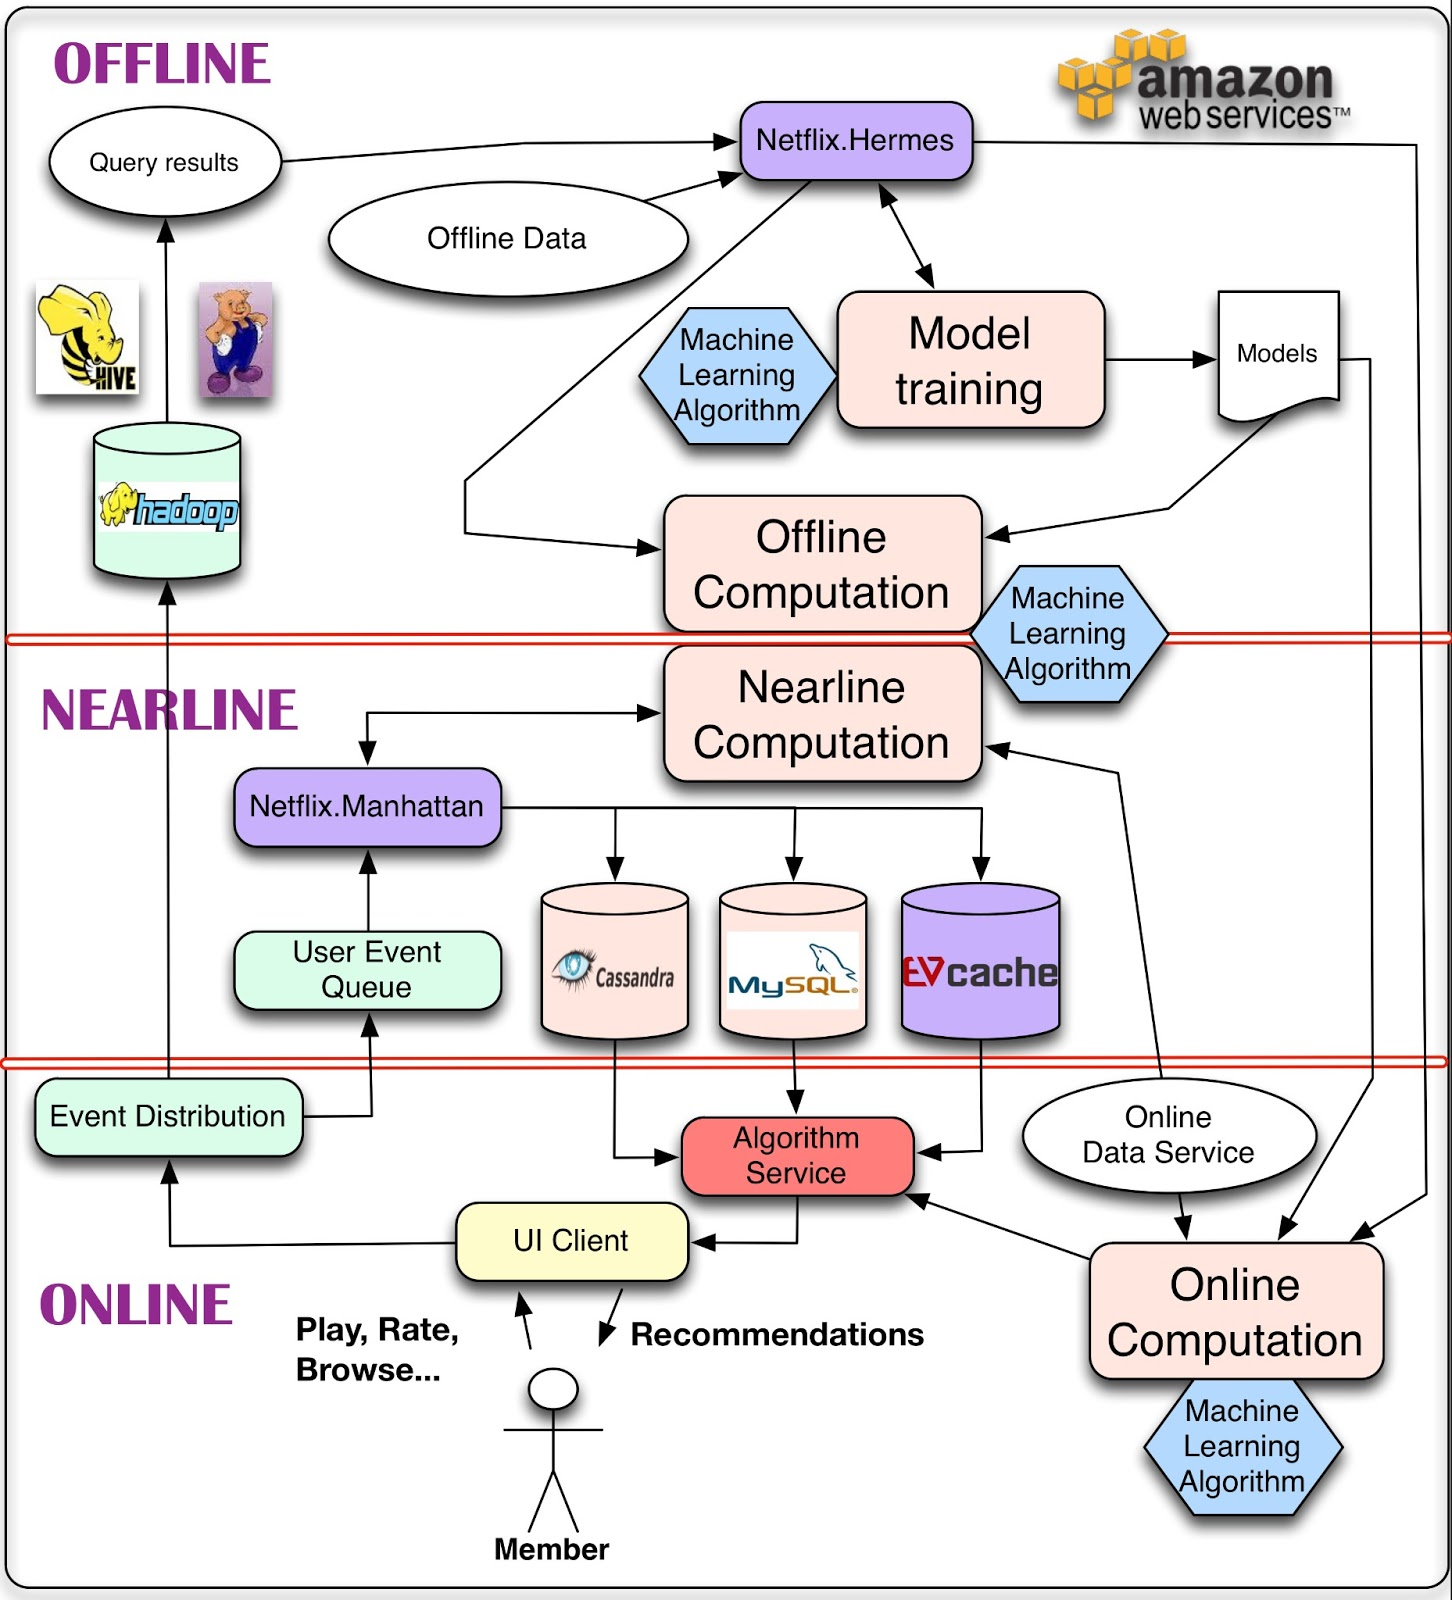
\includegraphics[width=0.4\linewidth]{assets/netflix-architecture.png}
  \caption{The Netflix architecture; suffice to say, it uses a lot of services}
  \source{https://netflixtechblog.com/system-architectures-for-personalization-and-recommendation-e081aa94b5d8}
  \label{fix:netflix-architecture}
\end{figure}

Would Netflix develop their entire system as a monolith and one aspect, say the movie recommendation algorithm, needs scaling, then two whole application requires duplication. It is highly cost-ineffective, especially for a company of that size with millions of users. With service-oriented architecture, just the part responsible for the recommendation algorithm needs to be scaled up. Because the scaling is limited in scope, only the right amount of additional computing power is used, saving the company much in infrastructure costs. Additionally, spinning up an instance of an entire application is usually complicated and time-consuming. But in big infrastructures such as Netflix, scaling happens in near-realtime with the help of algorithms ~\cite{netflix.2013}. It is, therefore, necessary to instantiate individual services as fast as possible to react to new demand in time.

\begin{figure}[ht]
  \centering
  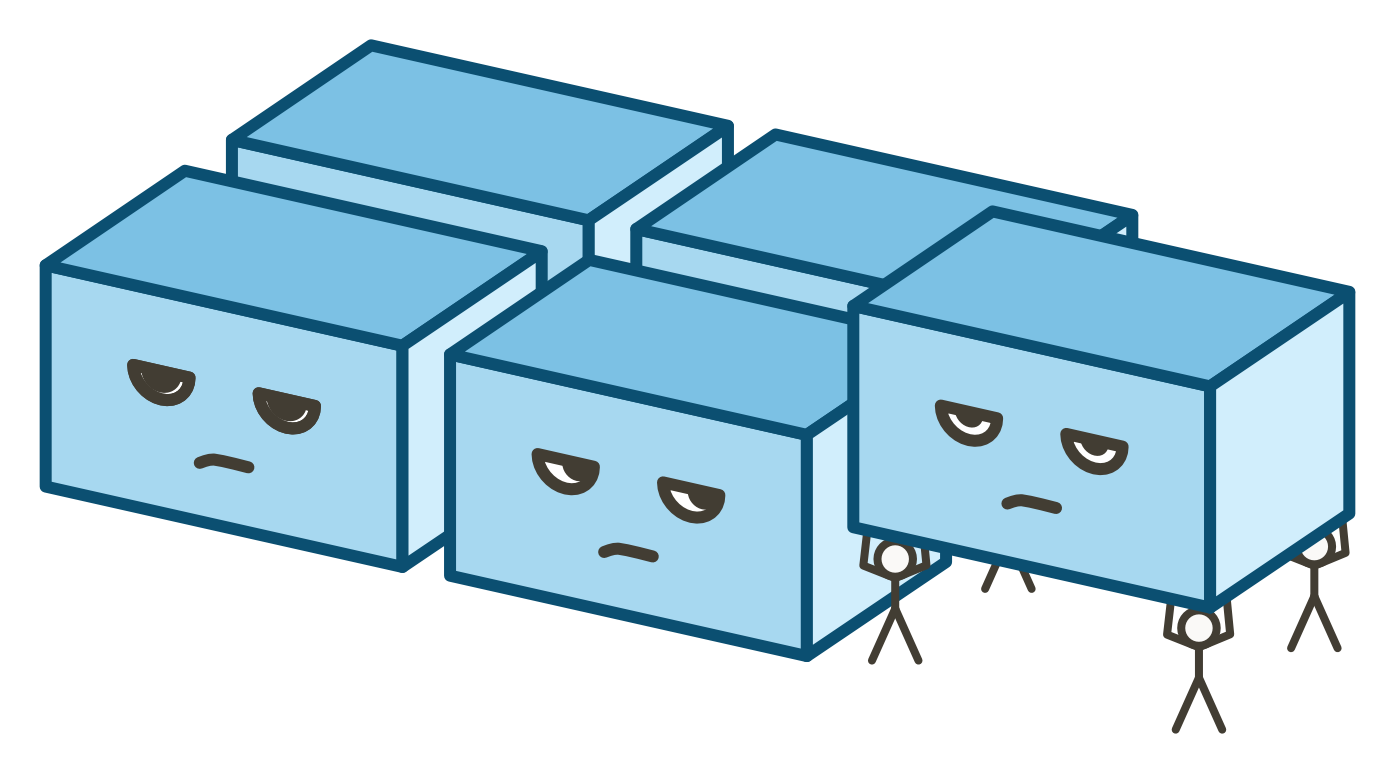
\includegraphics[width=0.55\linewidth]{assets/illustration-monolith-scaling.png}
  \caption{Monoliths can only be scaled as one block}
\end{figure}

Only a microservice architecture enables such granular scaling. On the other hand, the more services make up an application, the more intricate it becomes to operate. A company has to balance the overhead of complexity with the benefit of cost-savings in infrastructure. For this reason, smaller companies shouldn't start immediately with a granular service architecture. It may be more cost-effective to start with a monolith and break it up later, even if this means additional development time for refactoring.


\subsection{The right tool for the right job}

Distributed governance means that each team can choose the tool that fits their problem best. With monoliths, there is always a technology lock-in for the programming language and even frameworks and libraries. Microservices avoid this limitation by design. If, for example, the default technology stack for a software project is Java, but one service is using a machine learning model, this service can be written in Python for which more machine learning libraries are available.

There is but one catch, in the real world product managers don't like to employ new people but want to rely on existing skills. If teams change, it is essential for them that new team members can hit the ground running, which is easier if services use similar technologies. But even then, the flexibility to pick and choose libraries and frameworks best suited to the task is a massive win for the developer. The most significant time sink is usually legacy code and old dependencies, which can't be updated because some arcane part of the codebase is still using an outdated method. Microservices isolate such problems and speed up development.


%%
%% Challenges of implementing a microservice
%%
\section{Challenges of implementing a microservice}

\begin{itemize}
  \item \done{Complexity of ecosystem}
  \item \done{Design challenge because often monolith software is old and overcomplicated.}
\end{itemize}

There are three main challenges with the architectural style of microservices that require the developer to rethink some deign decitions. The data is distributed so the developer has to deal with eventual consistency .communication between services is expensive which requires more discipline and less greediness when requesting data. And the increased complexity of the infrastructure requires more resources in operations.


\subsection{Decentralized Data}
\label{sec:theory:challenges:data}

The probably greatest challenge with microservices is decentralized data management. As already noted in the section on page \pageref{sec:theory:decentralized-data}, it is unavoidable with microservices to have distributed databases. The challenge for the developers is to design the system, such as not to create data duplication. For example, almost every service usually needs access to user data. Think of an order or a shopping cart; it always has an assigned to a user. In monoliths, it is comparatively cheap to greedily query the database for the respective object together with its user. In a microservice environment, this cannot be done on the database level. Instead, the program iterates over all objects and request each user with an expensive API call from another service. There are solutions to parallelize these requests, which reduces the time for such operations tremendously. An example in JavaScript is the \inlinecode{Promise.all()} function which can handle parallel asynchronous calls in arrays ~\cite{mdn.2020}. But the better architectural ideal is to avoid them altogether.

\begin{figure}[ht]
  \centering
  
\includegraphics[width=0.55\linewidth]{assets/illustration-decentralized-data.png}
  \caption{Decentralized data is hard to manage}
\end{figure}

Let's use a shopping cart webpage as an illustration of how to deal with this constraint. In a traditional monolith, the server queries all data greedily from the database, assembles the page, and sends the assembled HTML template to the user. In a microservice environment, the page runs a JavaScript framework frontend, which needs to request all the data from the server. The frontend sends a request to the shopping cart service for the current state of the user's cart. The shopping card service could directly request the orders from the order component, but this would result in a more expensive request, making the user wait. Instead, the shopping cart component can answer with a list of order IDs. Not the frontend already knows how many orders it needs to display and can show placeholders to the user. There may be additional info in the service's response like the total amount payable, which the page can show already. Next, the frontend asks the order service API for all the orders by ID. As each order arrives, the frontend can fill the placeholder with actual information. The total loading time is a little longer than having the shopping cart service assemble the information directly, but it results in better user experience.

If services need to be scaled up and their databses duplicated then developers have to deal with "eventua consistency" ~\cite{fowler.2015}. It ca no longer assumed that data is consistend because write access for the same resource happens accross multiple databases simultaneously. Eventyally tha data will be synced between all database duplicates or managed by a master database, but at every given moment the developer has to assume that the data is not exactly consistent.

\begin{figure}[ht]
  \centering
  
\includegraphics[width=0.70\linewidth]{assets/youtube-view-counter.png}
  \caption{The YouTube view counter is an example for eventual consistency because of service oriented architecture}
  \source{https://www.youtube.com/watch?v=RY_2gElt3SA}
\end{figure}

An great example is the YouTube view counter. It is essential for YouTube to have a correct view count because it is essentially their internal currency and used to calculate advertisement revenue. But views occure in different countries all accross the world hitting many different servers. So the number off views each user sees can be different depending on the particular server they requested and the moment in time. But eventually all counts are tallied up and one authoritative number is calculated
~\cite{scott.2018}.


\subsection{Disciplined Communication}
\label{sec:theory:challenges:communication}

Inside a monolith, the individual components can call each other's methods to get information or trigger tasks. Because method calls are cheap, it doesn't matter very much how many method calls a specific task needs to make. It is also comparatively easy to understand other methods or even to add new ones as required.

\begin{figure}[ht]
  \centering
  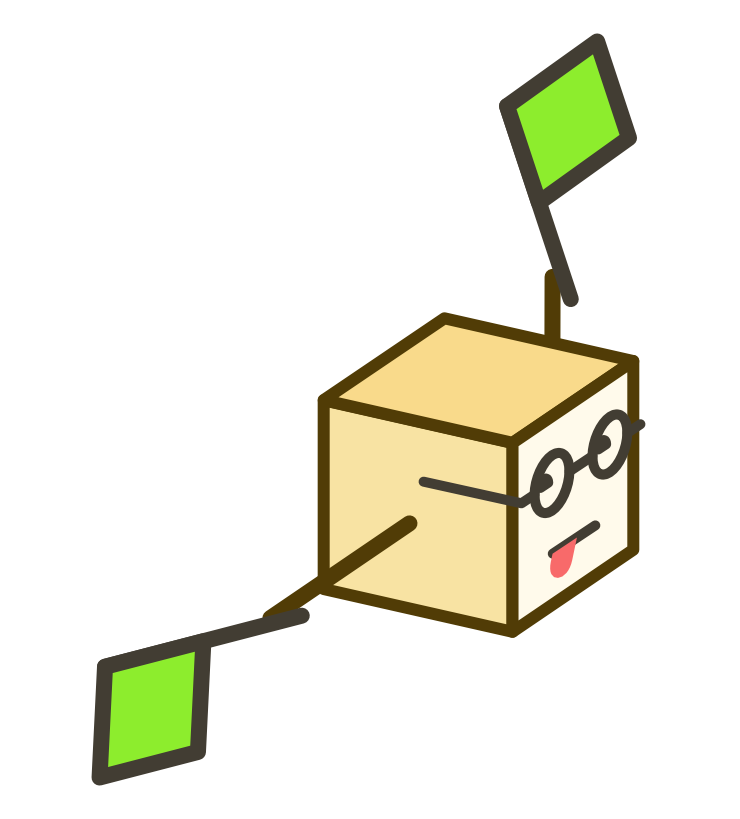
\includegraphics[width=0.25\linewidth]{assets/illustration-microservice-flags.png}
  \caption{Microservice communication requires more discipline}
\end{figure}

A microservice is essentially a black box with a public interface, an API. API calls are almost always HTTP requests using the internet to connect to the other end. The internet has an inherent latency, which usually is around 150-300 ms, an eternity for a computer. It means API calls are by magnitudes more expensive than simple method calls inside a program. It is, therefore, essential that developers think carefully when and how often other services are requested. It is especially crucial when not only one data point but a whole set is processed. As noted in the previous section, there are ways a programming language provides to parallelize such expensive tasks. But the better solution is to design the system in such a way as to minimize API requests or optimize tasks, so they are processes in smaller junks.


\subsection{Operational Complexity}
\label{sec:theory:challenges:ops}

Each service is deployed individually and requires its deployment pipeline, staging instance, version control, and error reporting ~\cite{fachat.2019.1}. In other words, the operational part of running and deploying the application is multiplied. Additionally, each service can use different technology, dependencies, and even third-party services. Because services nowadays run in the cloud, every instance is connected to the open internet. Thus authentication layers have to be managed, and services need permissions to call each other APIs and to access their respective databases. A bigger operations team is needed to manage the additional complexity. This point is one of the reasons why new projects should start as microservices and grow into service-oriented architectures as the need arises ~\cite{krivtsov.2019}.

\begin{figure}[ht]
  \centering
  
\includegraphics[width=0.25\linewidth]{assets/illustration-microservice-stack.png}
  \caption{Microservice architecutres require a mature ops team}
\end{figure}



%%
%% When does a microservice make sense?
%%
% \section{When does a microservice make sense?}

% \begin{itemize}
%   \item \todo{What type of application are microservices best suited for? (Scallable, defined scope)}
%   \item \todo{Good size of a team for a microservice}
%   \item \todo{When not to use distributed service architecture}
% \end{itemize}



%%
%% How to extract a microservice from an existing application?
%%
\section{How to extract a microservice from an existing application?}

\begin{itemize}
  \item \done{How to make a cut in a big application (monolith)}
\end{itemize}


\subsection{Justify Business Value}

A developer's time is not free for the company. When planning to extract a microservice from an existing application, the first question the company asks is: "Does this create value?" Why should the company allocate developer time to rewrite a functionality which already exists and is working? What is the additional value created for the company for the time spent creating the new service? It should be sufficiently clear by now that we can not argue with faster development. Yes, developing and extending a single microservice is quicker than building the same feature embedded in a monolith. And in the long-run development of new features as a whole may speed up. But at least in the beginning these gains are offset by the increased complexity\footnote{See page \pageref{sec:theory:challenges:ops}} and the more stringent requirements on data\footnote{See page \pageref{sec:theory:challenges:data}} and communication\footnote{See page \pageref{sec:theory:challenges:communication}}.

\begin{figure}[ht]
  \centering
  
\includegraphics[width=0.3\linewidth]{assets/illustration-business-values.png}
  \caption{Justify the business value of a microservice}
\end{figure}

The value chiefly lies in these three points, quicker release cycles, cheaper and easier scalability, and stronger resilience of the application. As already discussed in the section, "Why are microservices currently interesting?" on page \pageref{sec:theory:interesting} quick release cycles are interesting for applications that live in the cloud. They are also attractive to management who can show new features to users quickly. Scalability is the financially most persuasive argument. With growing numbers of users, the savings in infrastructure with services that can scale granularly are exponential.

Stronger resilience is built into the design of microservices if done right. It means that the system can continue to function with delays or even crashes of individual services. The Netflix Simian Army is a compilation of testing scripts like the Latency Monkey, induces artificial delays in a client-server communication, or the Chaos Monkey, randomly disabling production instances ~\cite{netflix.2011}. They have even a tool simulating an entire data center outage in the production environment. It is the stuff of developers' nightmares and in many companies cause for engineering team all-night and weekend shifts. At Netflix, they use these tools to incentive their programmers to build their services resilient in the first place. So if an outage or breakdown happens, other instances or datacenters dynamically scale to carry the load, and the user doesn't even realize anything happened.


\subsection{Define Boundaries}

Every monolith of sufficient size has natural boundaries. We want to find these boundaries and define them well enough to make a cut. Great engineering teams organize into smaller teams. For monoliths, teams consist of members with specific technological knowledge like database or backend code. The application reflects these separations in its codebase because developers seek the way of least resistance and try to solve tasks internally. This is an example of Conway's law in action, as quoted earlier\footnote{See page \pageref{sec:theory:what:capabilities}}. Figure \ref{fig:illustration-monolith-layers} shows the typical layer separations of an application. In most cases, there are three layers, the database, backend, and frontend. But there may also be service layers, data access object layers, routing layers, and others. However, when looking for boundaries inside monoliths, we are not looking for horizontal layers.

\begin{figure}[ht]
  \centering
  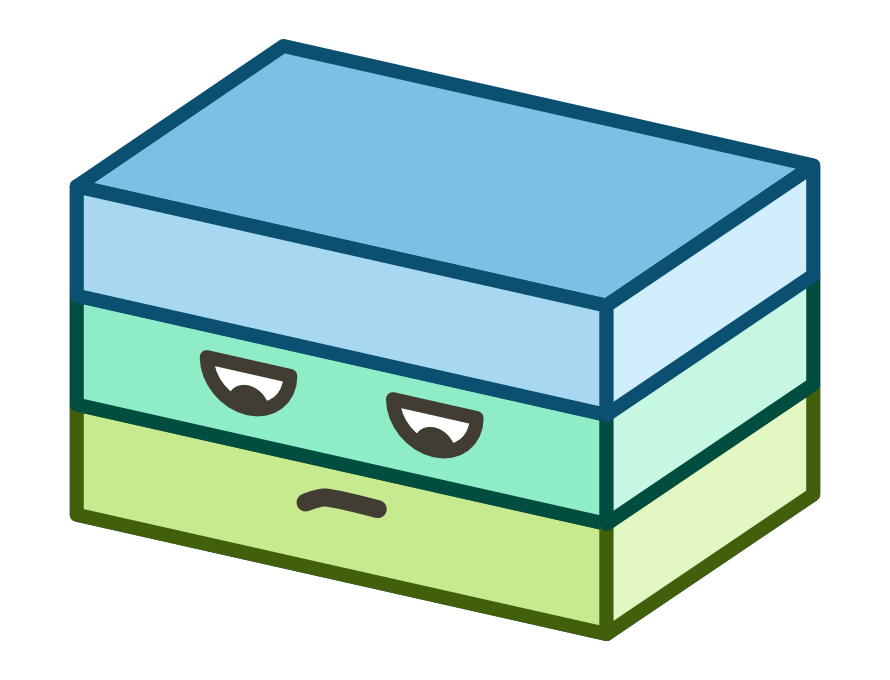
\includegraphics[width=0.4\linewidth]{assets/illustration-monolith-layers.png}
  \caption{Applications are usually divided by horizontal layers}
  \label{fig:illustration-monolith-layers}
\end{figure}

We are concerned with vertical boundaries that separate a monolith along business domain boundaries. Within the team, there are very likely already efforts to separate components of the code by business domains and to couple them as loosely as possible. There are always heavily coupled spaghetti code components and reasonably well-defined fringe components with only one or two dependencies. These loosely coupled, distinct components are our first target. Find the low-hanging fruit among the existing boundaries and start from there.

\begin{figure}[ht]
  \centering
  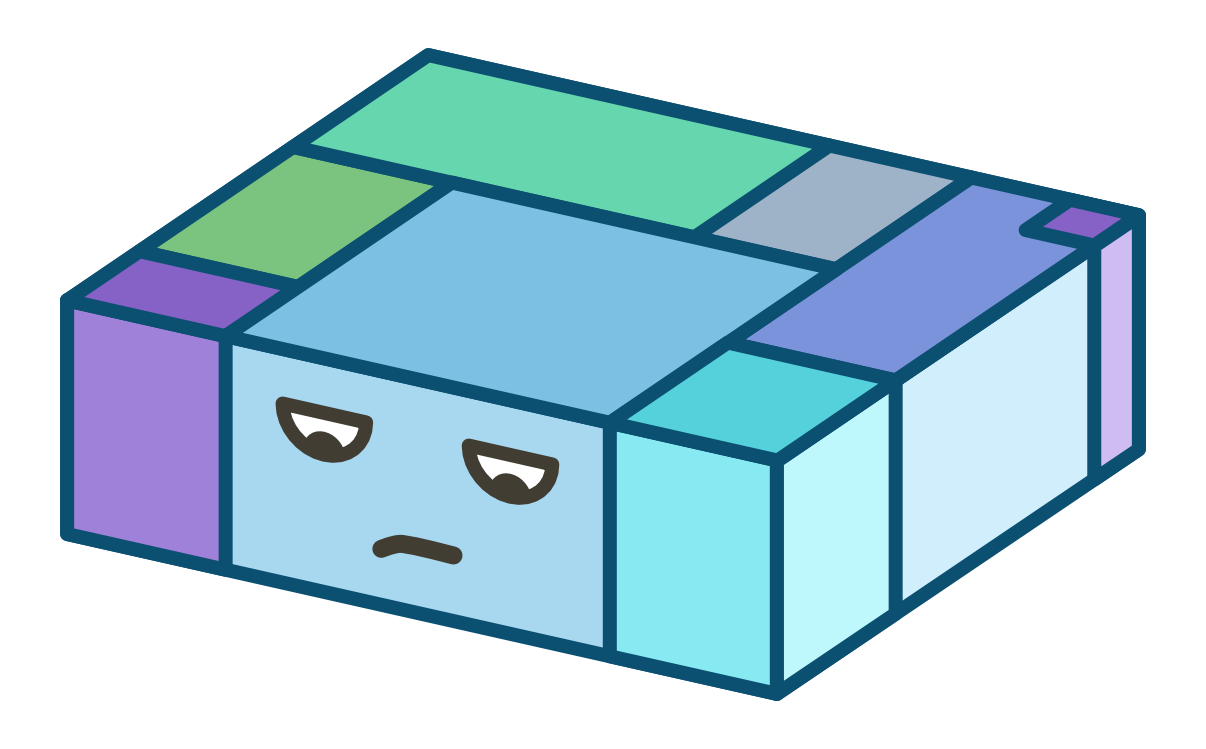
\includegraphics[width=0.4\linewidth]{assets/illustration-monolith-boundaries.png}
  \caption{Look for boundaries that already exist inside the monolith}
\end{figure}

Capgemini assigned me that task to exactly such a component. This part of the monolith is responsible for creating a printable PDF from a dataset passed to it. It is, if you will, the textbook example for a microservice because it was comparatively loosely coupled and very well defined. Chapter \ref{sec:arch} explains in more detail how I investigated and defined the boundaries of this specific component and then decided about the cuts.

\begin{figure}[ht]
  \centering
  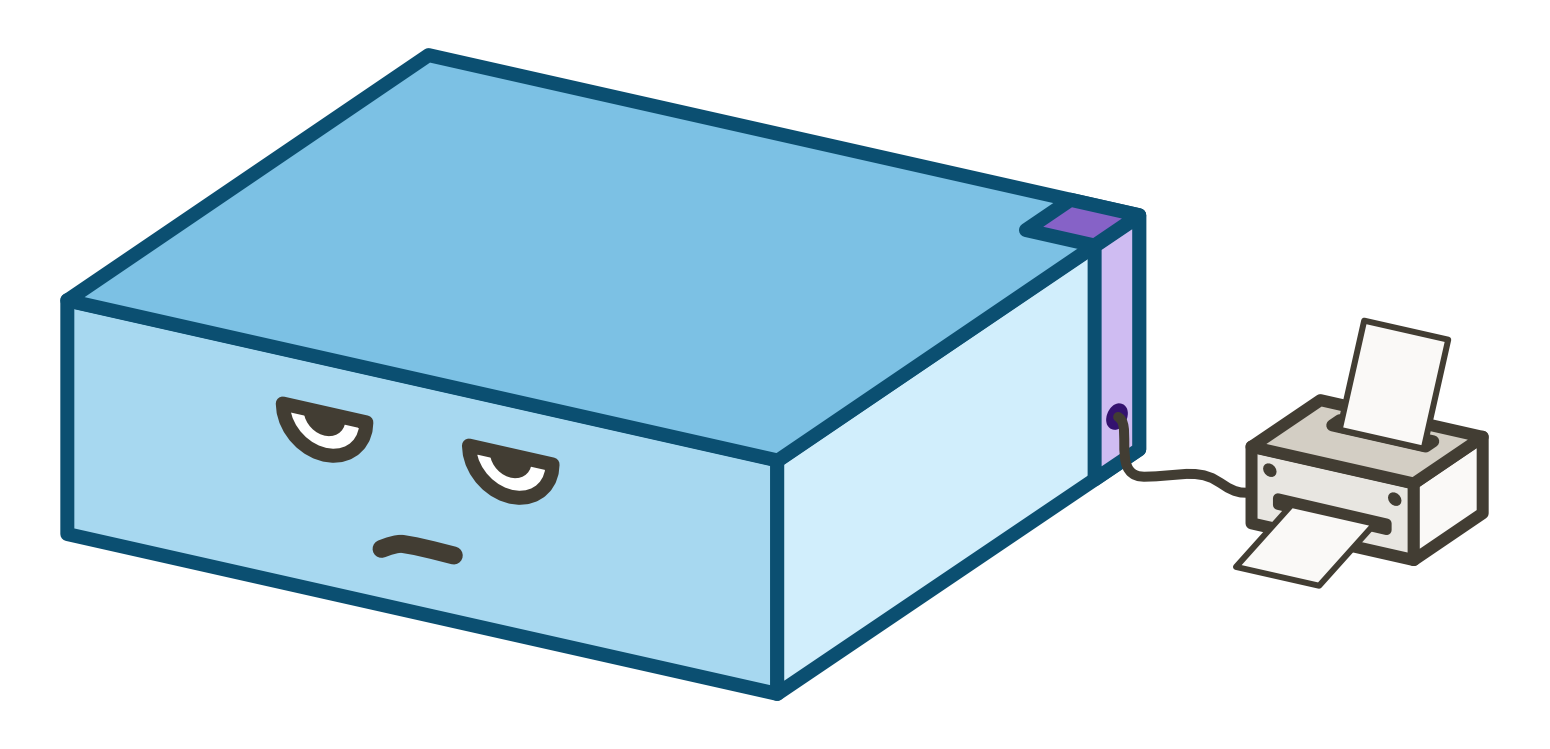
\includegraphics[width=0.4\linewidth]{assets/illustration-monolith-printer.png}
  \caption{One component inside the monolith is responsible for generating PDFs}
\end{figure}

Having defined the cuts for the first component, work yourself through the monolith incrementally. Note that it usually makes more sense to finish extracting one service before moving on to the next to take into account the learnings and changes from the process itself. In the ideal world, you could split up the monolith into equal parts, just like a pizza. In reality, their services differ vastly in size, and usually, there is one central service one cannot further reduce into smaller parts. As a guide, we can consider Jeff Bezos's "Two-Pizza rule," which says to keep teams and projects manageable, each team should not exceed the number of members two pizzas can feed ~\cite{hern.2018}. Ideally, no more than one team owns and runs a microservice, which gives us a good pointer for the maximum size of a microservice.


\subsection{Design API}

A comprehensive API documentation is addressing the challenge from page \pageref{sec:theory:challenges:communication} for "Disciplined Communication." A microservice is treated as a black box by other services because they should not know its inner workings. The only thing other services can and should know is how the public interface works. There are different ways services can communicate with one another. However, the primary way is through HTTP requests. Among HTTP requests, there are different conventions; this paper treats only the REST API convention because it is the most common standard to date.

\begin{figure}[ht]
  \centering
  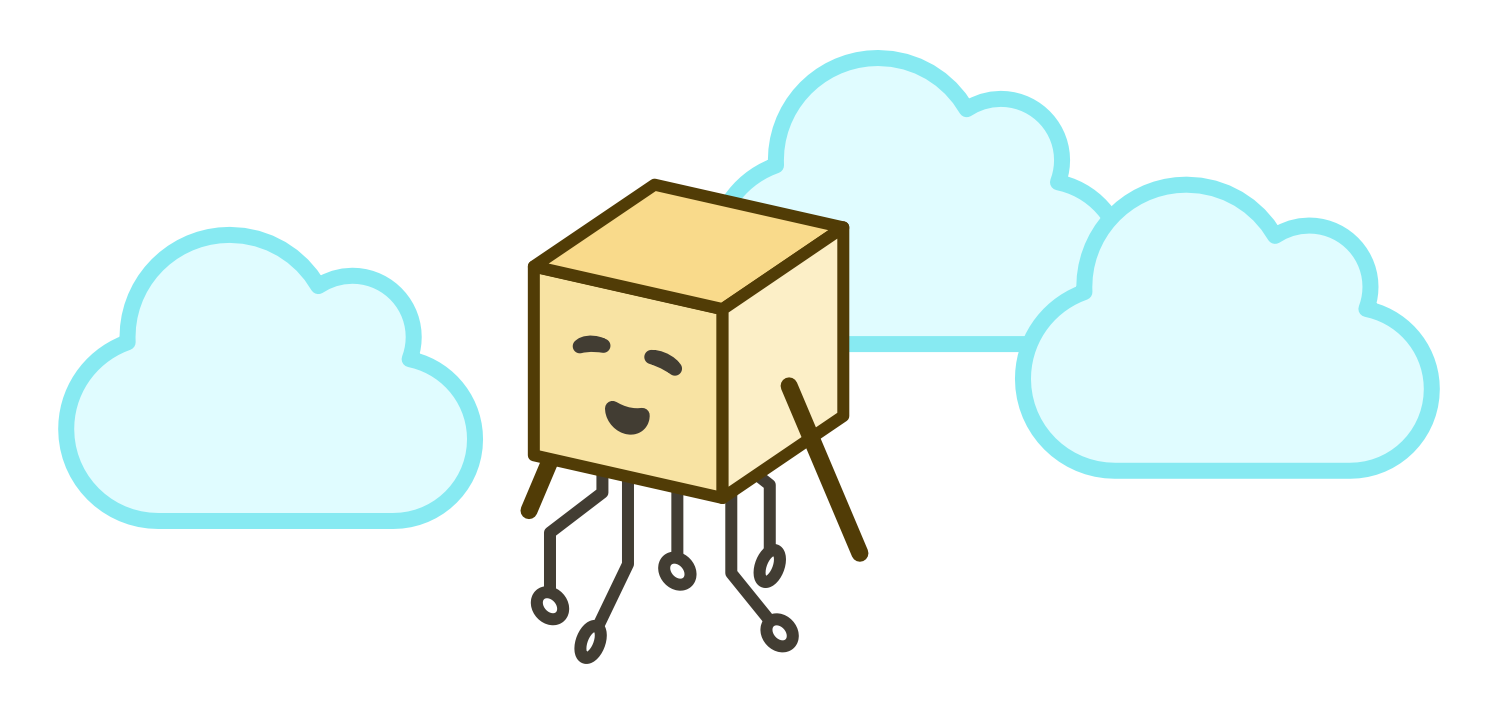
\includegraphics[width=0.55\linewidth]{assets/illustration-microservice-api.png}
  \caption{Good API documentation is key}
\end{figure}

REST stand for "Representational State Transfer" ~\cite{rest.2020}. A REST API follows three simple principles. It uses HTTP verbs like GET, POST, or DELETE to denote the action of the current request. It targets a resource with the URL of the request. For example, \inlinecode{/users/123} would target the user with ID \inlinecode{123}. And it uses status codes to respond to these requests so that machines can make sense from the response. For example, if the server responds with status code 200, it means the request was successful; if it responds with 404, it means that it couldn't find the resource, maybe because the user ID doesn't exist. An example HTTP request following the REST convention is \inlinecode{GET https://dog.ceo/api/breed/germanshepherd/images/random}, this requests a random image of from the \inlinecode{dog.ceo} API of the breed "German Shepherd." It is straightforward to try out any API by just pasting the URL into the browser address bar, see figure \ref{fig:dog-api}. The browser always performs a GET request by default.

\begin{figure}[ht]
  \centering
  \begin{subfigure}[b]{0.75\linewidth}
    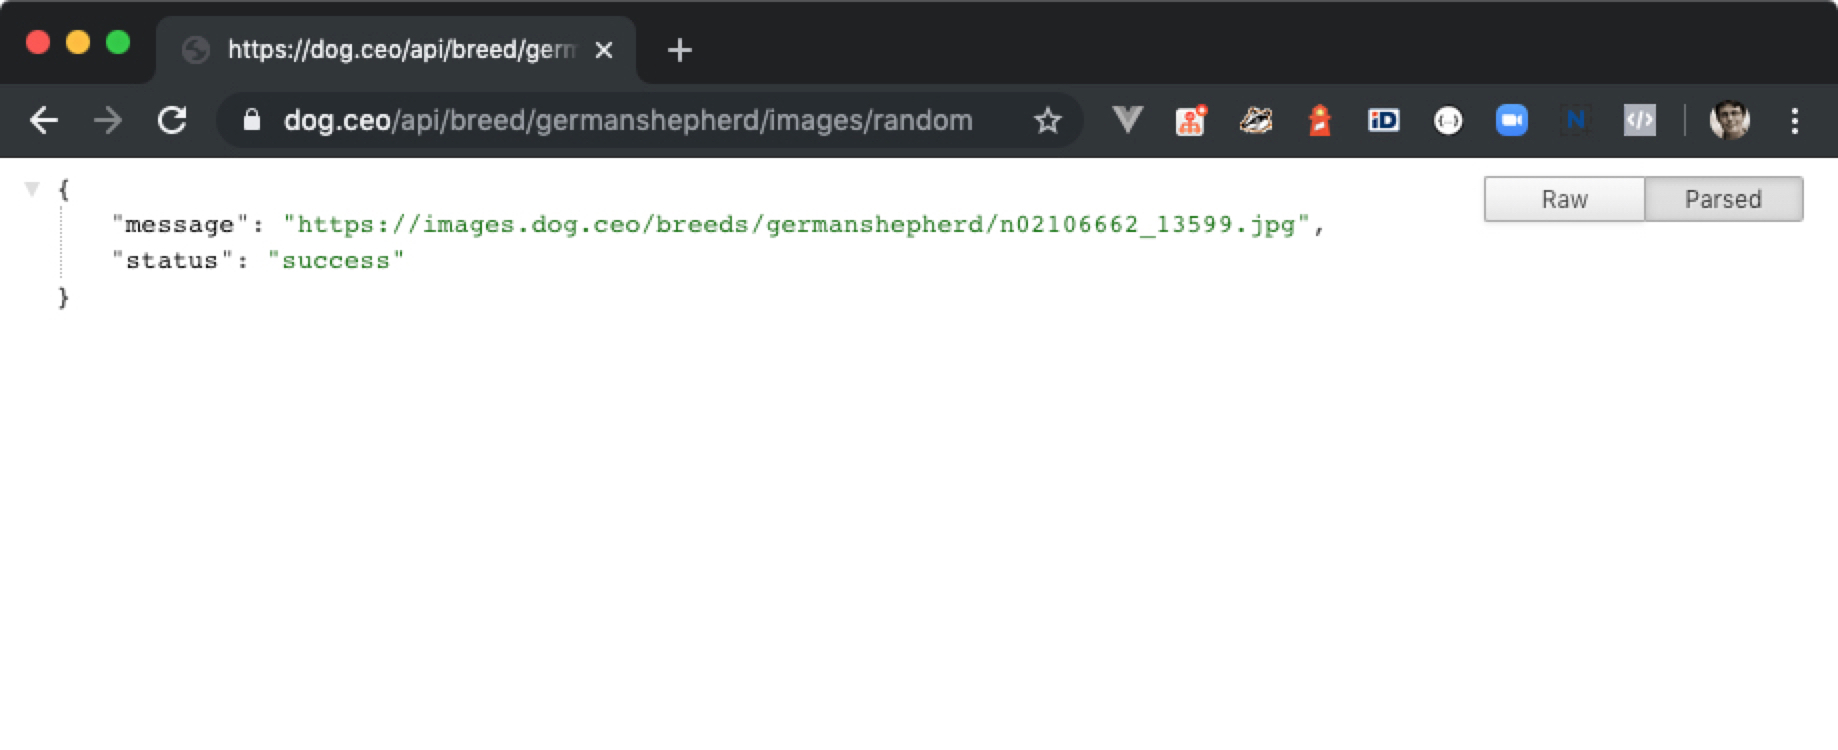
\includegraphics[width=\linewidth]{assets/dog-api-request.jpg}
  \end{subfigure}
  \begin{subfigure}[b]{0.75\linewidth}
    
\includegraphics[width=\linewidth]{assets/dog-api-image.jpg}
  \end{subfigure}
  \caption{Simple request to the dog.ceo API for a random German Shepherd}
  \label{fig:dog-api}
\end{figure}

Because the API is the only publicly accessible part of the application, it must be well documented. Meaning the documentation is complete, other teams know where to find it, and it lives with the application and doesn't become outdated. Nothing is more useless than documentation that is not up to date. For this reason, Swagger\footnote{See https://swagger.io/}, now in its third version called OpenAPI, is an excellent tool because it combines a standardized documentation format with an automatically generated webpage that is easy to use. And it is even possible to generate automatic code scaffolding from this documentation file; this way, the documentation becomes part of the development, which guarantees that it stays up to date.

While documentation is essential, the design of the API is no less important. The design here means to choose the right HTTP verbs and reasonable resource paths. Let's take a user resource as an example. It should be possible to request a list of all users, one specific user by its identifier and, let's say, all the orders a user made. Additionally, a list of all orders can be requested and again a single order by its identifier. The API routes would look something like this:

\begin{lstlisting}
/users                 -> get all users
/users/{userId}        -> get one user by userId
/users/{userId}/orders -> get all orders of one user by userId
/orders                -> get all orders
/order/{orderId}       -> get one order by oderId
\end{lstlisting}

It is also possible to define a route \inlinecode{/users/{userId}/orders/{orderId}}, but it's an unnecessary requirement to provide the userId if the oderId perfectly identifies an order. Chapter \ref{sec:impl:api} on page \pageref{sec:impl:api} looks at API design from the perspective of the practical implementation of the CEMicro\footnote{CEMicro is the name of the microservice the author developed as the practical part of this thesis} service.


\subsection{Develop Software}

After the crucial steps of justifying the business value, defining the boundaries, and designing the API of the new microservice, all the hard steps are taken. The last step is that of implementing the service itself. There are, of course, still decisions to be made like the choice of language, framework, and libraries. But because the boundaries are now well defined and with the API, it is clear what behavior is expected, the actual development is comparatively easy. Chapter \ref{sec:impl} of this paper deals at length with the minutia of the implementation of CEMicro.

\begin{figure}[ht]
  \centering
  
\includegraphics[width=0.2\linewidth]{assets/illustration-microservice-development.png}
  \caption{The development of a microservice is the easiest part}
\end{figure}



%%
%% Warp-up
%%
\section{Warp-up}

It is incorrect that there is a right or wrong way to design a system. A monolith doesn't need destructuring into services because it is the wrong architecture, but because the requirements outgrew its benefits. Once the concept is understood, and the monolith mapped out the actual work of cutting out microservices is not even that difficult. It turns out that understanding the boundaries and interfaces is the main work, part of it is, of course, the decision to which domain the data belongs. The conversation about implementation details and future possibilities takes up steam as soon as boundaries are easy to grasp.

I made this experience when demonstrating CEMicro to the project manager of the POS\footnote{POS is the short name of the point of sales application the department developed where I worked at Capgemini} project at Capgemini. The concept of configurable elements, the primary domain of CEMicro, is not easy to understand because it has many moving parts. However, once all present at the presentation caught a glimpse of the CEMicro design, that is, the user interface, the API, and the context diagram, immediately a healthy discussion commenced about specific pros and cons, better implementation details, and future possibilities. Rather than seeing this discussion as a critique, I was pleased to see that this complexity was suddenly so easy to grasp for everybody. I consider this a successful outcome of my work even if the result only represents a proof of concept.



